\documentclass[a4paper,11pt]{article}

% --- Paketit ---
\usepackage[utf8]{inputenc}
\usepackage[T1]{fontenc}
\usepackage[finnish]{babel}
\usepackage{amsmath, amssymb, amsthm}
\usepackage{geometry}
\geometry{left=3cm, right=3cm, top=3cm, bottom=3cm}

% --- Grafiikka ja kuvaajat (TikZ & PGFPlots) ---
\usepackage{tikz}
\usepackage{pgfplots}
\pgfplotsset{compat=1.18}
\usepgfplotslibrary{fillbetween}

% --- Tyyliasetukset ---
\setlength{\parindent}{0pt}
\setlength{\parskip}{1em}
\linespread{1.1}

% --- Otsikointi ---
\title{Optimointimallin matemaattinen johto}
\author{Elias Ervamaa}
\date{\today}

\begin{document}

\maketitle

\section{Johdanto}
Tässä dokumentissa johdetaan analyyttinen ratkaisu kahden jonon resurssien allokointiongelmalle. Tarkastelu etenee kahdessa vaiheessa: ensin johdetaan yksittäisen M/M/1-jonon odotusajan lauseke, minkä jälkeen ratkaistaan optimointiongelma Lagrangen kertoimien menetelmällä.

\subsection{Muuttujat}
Mallissa käytetään seuraavia merkintöjä:
\begin{itemize}
    \item $\lambda_i \in \mathbb{N}$: Saapumisintensiteetti (asiakasta / aikayksikkö).
    \item $\mu_i \in \mathbb{R}_+$: Palvelunopeus (palvelua / aika / työntekijä).
    \item $x_i \in \mathbb{R}_+$: Työntekijöiden määrä.
    \item $w_i \in \mathbb{R}_+$: Odotusajan painokerroin ("haittakerroin").
    \item $c_i \in \mathbb{R}_+$: Työntekijän yksikkökustannus.
    \item $B \in \mathbb{R}_+$: Kokonaisbudjetti.
\end{itemize}

\newpage
\section{Todennäköisyysjakaumat}

\subsubsection*{Saapumisprosessi (Poisson)}
Asiakkaiden saapuminen noudattaa Poisson-prosessia. Todennäköisyys sille, että aikayksikössä ($t$) saapuu tasan $k$ asiakasta, on:
\begin{equation}
    P(X=k) = \frac{\lambda^k e^{-\lambda}}{k!}, \quad k = 0, 1, 2, \dots
\end{equation}

\begin{center}
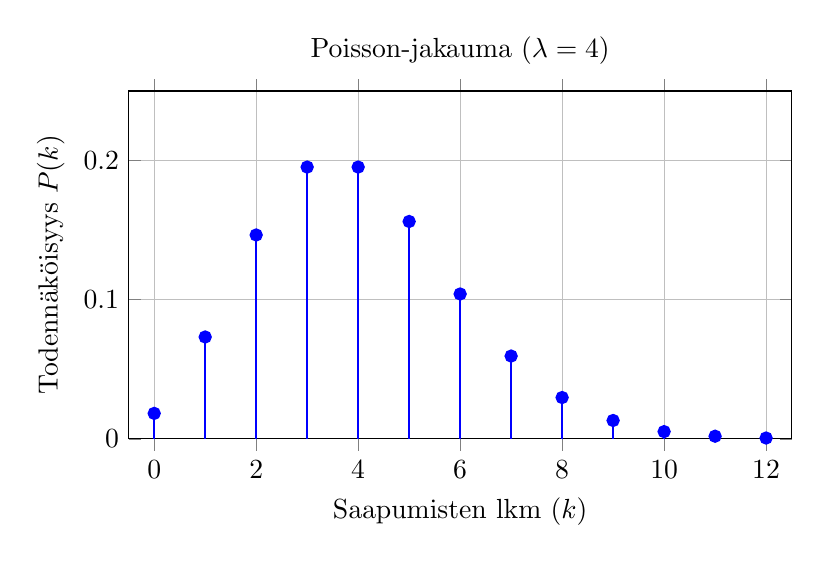
\begin{tikzpicture}
\begin{axis}[
    width=10cm, height=6cm,
    title={Poisson-jakauma ($\lambda=4$)},
    xlabel={Saapumisten lkm ($k$)},
    ylabel={Todennäköisyys $P(k)$},
    ymin=0, ymax=0.25,
    xmin=-0.5, xmax=12.5,
    ybar,
    bar width=2pt,
    grid=major
]
    \addplot+[ycomb, blue, thick, mark=*] coordinates {
        (0, 0.0183) (1, 0.0732) (2, 0.1465) (3, 0.1953) (4, 0.1953)
        (5, 0.1562) (6, 0.1041) (7, 0.0595) (8, 0.0297) (9, 0.0132)
        (10, 0.0052) (11, 0.0019) (12, 0.0006)
    };
\end{axis}
\end{tikzpicture}
\end{center}

\subsubsection*{Palveluajat (Eksponentti)}
Palveluajat $T$ noudattavat eksponenttijakaumaa. Tiheysfunktio on:
\begin{equation}
    f(t; \mu) = \mu e^{-\mu t}, \quad t \ge 0
\end{equation}
Tässä $\mu$ kuvaa palvelunopeutta (rate), joten keskimääräinen palveluaika on $E[T] = 1/\mu$.

\begin{center}
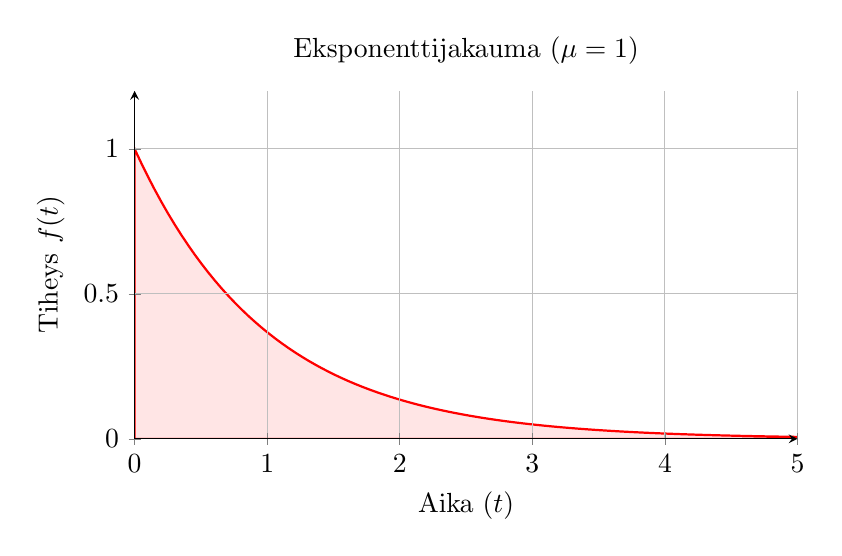
\begin{tikzpicture}
\begin{axis}[
    width=10cm, height=6cm,
    title={Eksponenttijakauma ($\mu=1$)},
    xlabel={Aika ($t$)},
    ylabel={Tiheys $f(t)$},
    domain=0:5, samples=100,
    ymin=0, ymax=1.2,
    axis lines=left,
    grid=major,
    axis on top
]
    \addplot [thick, red, fill=red!10] {exp(-x)} \closedcycle;
\end{axis}
\end{tikzpicture}
\end{center}

\newpage

\section{M/M/1-jonon johtaminen}

Tarkastellaan yhtä jonoa. Määritellään liikennekuorma $\rho = \frac{\lambda}{x\mu}$.

\subsection{Tasapainoehto}

Jotta jono pysyisi tasapainotilassa eikä kasvaisi rajatta, on $x > \frac{\lambda}{\mu}$ (eli $\rho < 1$). Oletetaan, että on kulunut tietty aika, jonka jälkeen jonon jakauma on vakaassa tilassa:

\begin{align*}
    \intertext{Tasapainoehto tilojen $n-1$ ja $n$ välillä (sisäänvirtaus = ulosvirtaus):}
    \lambda p_{n-1} &= (x \mu) p_n \\
    p_n &= \frac{\lambda}{x \mu} p_{n-1} = \rho p_{n-1} \\
    \intertext{Iteroimalla tätä rekursiota alkaen tilasta $n=0$ saadaan yleinen termi:}
    p_n &= \rho^n p_0 \\
    \intertext{Koska todennäköisyyksien summan täytyy olla 1, saamme äärettömän geometrisen sarjan:}
    \sum_{n=0}^{\infty} p_n &= p_0 \sum_{n=0}^{\infty} \rho^n = 1 \\
    \intertext{Kun $\rho < 1$, geometrinen sarja suppenee arvoon $\frac{1}{1-\rho}$. Ratkaistaan $p_0$:}
    p_0 \cdot \frac{1}{1-\rho} &= 1 \quad \implies \quad p_0 = 1 - \rho \\
    \intertext{Tällöin lopullinen todennäköisyysjakauma jonon pituudelle $n$ on:}
    p_n &= (1-\rho)\rho^n
\end{align*}

\vspace{1cm}

\subsection{Odotettu asiakasmäärä $L$}

Olkoon satunnaismuuttuja $N$ asiakkaiden lukumäärä systeemissä. Äsken johdettu $p_n$ on muuttujan $N$ todennäköisyysfunktio, eli $P(N=n) = p_n$.
Odotusarvo lasketaan summaamalla jokainen tila painotettuna niiden todennäköisyyksillä:
\begin{equation}
    L = E[N] = \sum_{n=0}^{\infty} n p_n = (1-\rho) \sum_{n=0}^{\infty} n \rho^n
\end{equation}

Summan $\sum n \rho^n$ laskemiseksi tarkastellaan tuttua geometrista sarjaa funktiota:
\begin{equation*}
    \sum_{n=0}^{\infty} x^n = \frac{1}{1-x}, \quad |x| < 1
\end{equation*}
Derivoidaan yhtälö puolittain muuttujan $x$ suhteen:
\begin{align*}
    \frac{d}{dx} \sum_{n=0}^{\infty} x^n &= \frac{d}{dx} (1-x)^{-1} \\
    \sum_{n=1}^{\infty} n x^{n-1} &= (-1)(1-x)^{-2}(-1) = \frac{1}{(1-x)^2}
\end{align*}
Kerrotaan puolittain $x$:llä, jolloin saadaan haluttu muoto:
\begin{equation}
    \sum_{n=1}^{\infty} n x^n = \frac{x}{(1-x)^2}
\end{equation}

Sijoitetaan tämä tulos (missä $x=\rho$) alkuperäiseen odotusarvon lausekkeeseen:
\begin{align*}
    L &= (1-\rho) \cdot \frac{\rho}{(1-\rho)^2} \\
    L &= \frac{\rho}{1-\rho}
\end{align*}

Palautetaan alkuperäiset muuttujat sijoittamalla $\rho = \frac{\lambda}{x\mu}$:
\begin{equation}
    L(x) = \frac{\frac{\lambda}{x\mu}}{1 - \frac{\lambda}{x\mu}} = \frac{\lambda}{x\mu - \lambda}
\end{equation}

Eli odotettu asiakasmäärä on: $\frac{\lambda}{x\mu - \lambda}$


% TÄHÄN TULEE LOPPUTULOS W(x) (Little's Law)

\newpage

\section{Optimointiongelma}

\subsection{Ongelman asettelu}
Minimoitava tavoitefunktio ja rajoitteet:

% TÄHÄN TULEE KAAVAT

\vspace{3cm}

\subsection{Lagrangen menetelmä}

Muodostetaan Lagrangen funktio $\mathcal{L}(x_1, x_2, \alpha)$:

% TÄHÄN TULEE LAGRANGEN FUNKTIO

\vspace{3cm}

Ratkaistaan KKT-ehdot (osittaisderivaatat nollaksi):

% TÄHÄN TULEE DERIVOINTI JA YHTÄLÖRYHMÄN RATKAISU

\vspace{8cm}

\subsection{Lopputulos}

% TÄHÄN TULEE LOPULLISET KAAVAT

\end{document}